\subsection{Sudoku puzzle}

Sudoku puzzle is a 9*9 grid with some cells filled, some are left to be found:

\newcounter{row}
\newcounter{col}

\newcommand\setrow[9]{
  \setcounter{col}{1}
  \foreach \n in {#1, #2, #3, #4, #5, #6, #7, #8, #9} {
    \edef\x{\value{col} - 0.5}
    \edef\y{9.5 - \value{row}}
    \node[anchor=center] at (\x, \y) {\n};
    \stepcounter{col}
  }
  \stepcounter{row}
}

\begin{center}
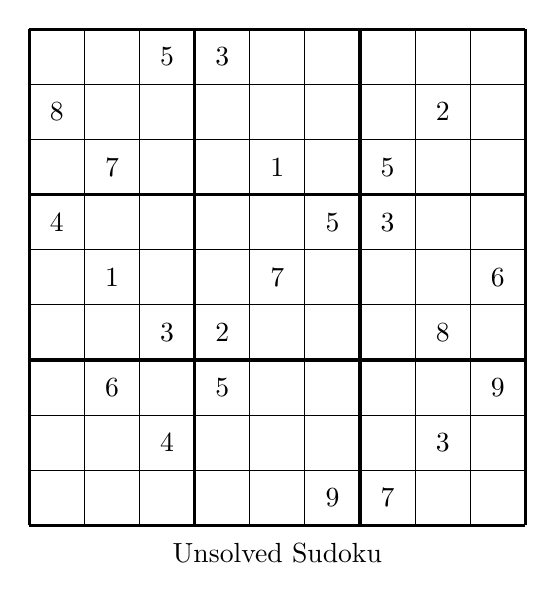
\begin{tikzpicture}[scale=.7]
  \begin{scope}
    \draw (0, 0) grid (9, 9);
    \draw[very thick, scale=3] (0, 0) grid (3, 3);

    \setcounter{row}{1}
    \setrow { }{ }{5}  {3}{ }{ }  { }{ }{ }
    \setrow {8}{ }{ }  { }{ }{ }  { }{2}{ }
    \setrow { }{7}{ }  { }{1}{ }  {5}{ }{ }

    \setrow {4}{ }{ }  { }{ }{5}  {3}{ }{ }
    \setrow { }{1}{ }  { }{7}{ }  { }{ }{6}
    \setrow { }{ }{3}  {2}{ }{ }  { }{8}{ }

    \setrow { }{6}{ }  {5}{ }{ }  { }{ }{9}
    \setrow { }{ }{4}  { }{ }{ }  { }{3}{ }
    \setrow { }{ }{ }  { }{ }{9}  {7}{ }{ }

    \node[anchor=center] at (4.5, -0.5) {Unsolved Sudoku};
  \end{scope}
\end{tikzpicture}
\end{center}

Numbers of each row must be unique, i.e., must contain all 9 numbers in range of 1..9 without repetition.
Same story for each column and also for each 3*3 square.

This puzzle is good candidate to try SMT solver on, because it's essentially an unsolved system of equations.

\subsubsection{The first idea}

The only thing we must solve is that how to determine in one expression, if the input 9 variables has all 9 unique numbers?
They are not ordered or sorted, after all.

From the school-level mathematics, we can devise this idea:

\begin{equation}
\underbrace{10^{i_1} + 10^{i_2} + \cdots + 10^{i_9}}_9 = 1111111110
\end{equation}

Take each input variable, calculate $10^i$ and sum them all.
If all input values are unique, each will be settled at its own place.
Even more than that: there will be no holes, i.e., no skipped values.
So, in case of Sudoku, 1111111110 number will be final result, indicating that all 9 input variables are unique, in range of 1..9.

Exponentiation is heavy operation, can we use binary operations? Yes, just replace 10 with 2:

\begin{equation}
\underbrace{2^{i_1} + 2^{i_2} + \cdots + 2^{i_9}}_9 = 1111111110_2
\end{equation}

The effect is just the same, but the final value is in base 2 instead of 10.

Now a working example:

\lstinputlisting{SMT/sudoku_plus.py}

\begin{lstlisting}
\$ time python sudoku_plus.py
1 4 5 3 2 7 6 9 8
8 3 9 6 5 4 1 2 7
6 7 2 9 1 8 5 4 3
4 9 6 1 8 5 3 7 2
2 1 8 4 7 3 9 5 6
7 5 3 2 9 6 4 8 1
3 6 7 5 4 2 8 1 9
9 8 4 7 6 1 2 3 5
5 2 1 8 3 9 7 6 4

real    0m11.717s
user    0m10.896s
sys     0m0.068s
\end{lstlisting}

Even more, we can replace summing operation to logical OR:

\begin{equation}
\underbrace{2^{i_1} \vee 2^{i_2} \vee \cdots \vee 2^{i_9}}_9 = 1111111110_2
\end{equation}

% FIXME: только часть исходника + ссылка на github
\lstinputlisting{SMT/sudoku_or.py}

Now it works much faster. Z3 handles OR operation over bit vectors better than addition?

\begin{lstlisting}
\$ time python sudoku_or.py
1 4 5 3 2 7 6 9 8
8 3 9 6 5 4 1 2 7
6 7 2 9 1 8 5 4 3
4 9 6 1 8 5 3 7 2
2 1 8 4 7 3 9 5 6
7 5 3 2 9 6 4 8 1
3 6 7 5 4 2 8 1 9
9 8 4 7 6 1 2 3 5
5 2 1 8 3 9 7 6 4

real    0m1.429s
user    0m1.393s
sys     0m0.036s
\end{lstlisting}

The puzzle I used as example is dubbed as one of the hardest known
\footnote{\url{http://www.mirror.co.uk/news/weird-news/worlds-hardest-sudoku-can-you-242294}} (well, for humans).
It took ~1.4 seconds on my Intel Core i3-3110M 2.4GHz notebook to solve it. % FIXME tilde

\subsubsection{The second idea}

My first approach is far from effective, I did what first came to my mind and worked.
Another approach is to use \texttt{distinct} command from SMTLIB, which tells Z3 that some variables (of unspecific number) must be distinct (or unique).
This command is also available in Z3 Python interface.

I've rewritten my first Sudoku solver, now it operates over \textit{Int} \textit{sort}, it has \texttt{distinct} commands instead of bit operations,
and now also other constaint added: each cell value must be in 1..9 range, because, otherwise, Z3 will offer (although correct) solution with too big
and/or negative numbers.

% FIXME: только часть исходника + ссылка на github
\lstinputlisting{SMT/sudoku2.py}

\begin{lstlisting}
\$ time python sudoku2.py
1 4 5 3 2 7 6 9 8
8 3 9 6 5 4 1 2 7
6 7 2 9 1 8 5 4 3
4 9 6 1 8 5 3 7 2
2 1 8 4 7 3 9 5 6
7 5 3 2 9 6 4 8 1
3 6 7 5 4 2 8 1 9
9 8 4 7 6 1 2 3 5
5 2 1 8 3 9 7 6 4

real    0m0.382s
user    0m0.346s
sys     0m0.036s
\end{lstlisting}

That's much faster.

\subsubsection{Conclusion}

The awesomeness of SMT-solvers is that our Sudoku solver has nothing else, we have just defined relationships between variables (cells).

\subsubsection{Homework}

As it seems, true Sudoku puzzle is the one which has only one solution.
The piece of code I've included in this article shows only the first one.
Using the method described earlier (\ref{SMTEnumerate}, also called ``model counting''), 
try to find more solutions, or prove that the solution you have just found is the only one possible.

\subsubsection{Further reading}

\url{http://www.norvig.com/sudoku.html}

\subsubsection{Sudoku as SAT problem}

It's also possible to represend Sudoku puzzle as a huge \ac{CNF} equation and use SAT-solver to find solution, but it's just trickier.

Some articles about it\footnote{Another one: \url{http://ocw.mit.edu/courses/electrical-engineering-and-computer-science/6-005-elements-of-software-construction-fall-2011/assignments/MIT6_005F11_ps4.pdf}}: \cite{Sudoku1}, \cite{Sudoku2}, \cite{Sudoku3}.

SMT-solver can also use SAT-solver in its core, so it does all mundane translating work.
As a ``compiler'', it may not do this in the most efficient way, though.

